\documentclass[12pt]{article}
\usepackage[left=2cm,top=2cm,right=2cm, bottom=2cm]{geometry}
\usepackage{parskip}
\setlength{\parskip}{0.5cm}
\usepackage[pdfborder=0,colorlinks=true,linkcolor=black,urlcolor=blue]{hyperref}
\usepackage{graphicx}
\usepackage{multirow}
% Note: fancyvrb does not come installed with the standard MiKTeX install and must be installed through the
%       package manager
\usepackage{fancyvrb}
% Note: sectsty does not come installed with the standard MiKTeX install and must be installed through the
%       package manager
\usepackage{sectsty}
\allsectionsfont{\sffamily}


\title{Universal Peer to Peer Community Creation Guide}
\author{Alexander Craig \and Alan Davoust \and Neal Arthorne \and Michael Yartsev }
\date{\today}

\begin{document}
\sffamily

% ------------------------------- TITLE PAGE -------------------------------
\begin{titlepage}
\begin{center}
\vspace*{1cm}

\includegraphics{img/up2p_title.png}\\
\textbf{\Huge{User's Guide}}\\
\vspace*{2cm}
Alexander Craig\\
Alan Davoust\\
Neal Arthorne\\
Michael Yartsev\\
\vspace*{2cm}
\today
\end{center}
\vfill
\begin{flushleft}
U-P2P was created by Babak Esfandiari, Aloke Mukherjee and Neal Arthorne in the Department of Systems and Computer Engineering, Carleton University, Ottawa, Ontario, Canada.\\
\vspace*{1cm}
\textbf{Additional development contributions from:}\\
Shawn Henry, Andrew N. Ravindran, Mayuran Subramaniam, Michael Yartsev, Alan Davoust, Alexander Craig\\
\vspace*{1cm}
\textbf{Carleton University}\\
The Department of Systems and Computer Engineering\\
1125 Colonel By Drive\\
Carleton University\\
Ottawa, Ontario\\
K1S 5B6\\
Canada\\
+1 613 520 5740 (Voice)\\
+1 613 520 5727 (Fax)\\
\textbf{\copyright 2003-2010 Carleton University}
\end{flushleft}
\thispagestyle{empty} 
\end{titlepage}

% ------------------------------- TABLE OF CONTENTS -------------------------------
\tableofcontents
\newpage

% ------------------------------- INTRODUCTION -------------------------------
\section{Introduction}
Universal Peer to Peer (U-P2P) is an XML and web based peer to peer file sharing framework. U-P2P uses XML meta-data to describe user defined arbitrary data types which can then be easily searched and shared through a simple web browser interface. U-P2P can be used to share anything from simple image or music files to complex and dynamic content such as flash games or Wiki articles. This is achieved by allowing content creators to share special assets which describe how a specific data type should be processed, stored, and displayed to users. U-P2P offers a simple interface to a highly flexible distributed network where every peer is also a content creator. U-P2P is an open source system working with the Gnutella protocol that you may modify to suit your own needs. This guide will give more details on the system and the concepts that it is based on, and covers some more practical issues such as installation and troubleshooting.

Data in U-P2P is shared as XML meta-data documents which may have any number of arbitrary file attachments. A simple example would be a music file stored in an mp3 file and attached to the following XML document:

\begin{SaveVerbatim}{verb:IntroExample}
<MyMusic>
	<title>Under The Boardwalk</title>
	<artist>The Drifters</artist>
	<duration>2:28</duration>
	<bitrate>128</bitrate>
	<file>file:undertheboardwalk.mp3</file>
</MyMusic>
\end{SaveVerbatim}
\fbox{
	\BUseVerbatim{verb:IntroExample}
}

In order to share a new type of data on the U-P2P network a user must create a "community" which describes the data type. The community definition includes properties describing the data type to be shared, as well as properties of the community itself (such as a description, category, tags, etc.). The community definition contains an XML schema that the data type's meta-data must match, as well as XSLT and CSS stylesheets, HTML pages, and any other arbitrary attachments which are needed to process, search for, and display the community's resources. These community definitions are stored in XML files and shared just like any other resource through the U-P2P "`Root Community".

Before a peer can share a specific data type they must join the community corresponding to the desired data type. The community definition is downloaded from the network to the peer's local U-P2P node. This includes any community attachments which are required to process, search for, and display the data type. Once a peer joins a community they are able to search the network for resources shared by other peers in the same community, and any locally stored resources will be shared with all other peers in the same community. Each U-P2P peer can be a member of any number of communities, and therefore can share many data types in parallel. Network searches are propagated only to those nodes which have subscribed to the community being searched, and many communities can be shared through the same network infrastructure.

Since resources are shared along with XML meta-data searches can be performed which are highly specific to the resource in question. For example, a node serving a photography community may allow users to search for images based on the brand of camera used, the resolution of the image, or the date a photograph was taken. The same node could simultaneously serve a wiki article community which allowed for searches based on article versioning history, or searches based on the cross-references between articles. The searchable terms of a community are defined by the content creator of the community. U-P2P provides built in facilities to perform text searches on article meta-data, as well as searches based on relational links between resources (For example, a community representing a database of actors may support searches such as "find all actors who have co-starred with Burt Reynolds").

\begin{figure}
  \centering
    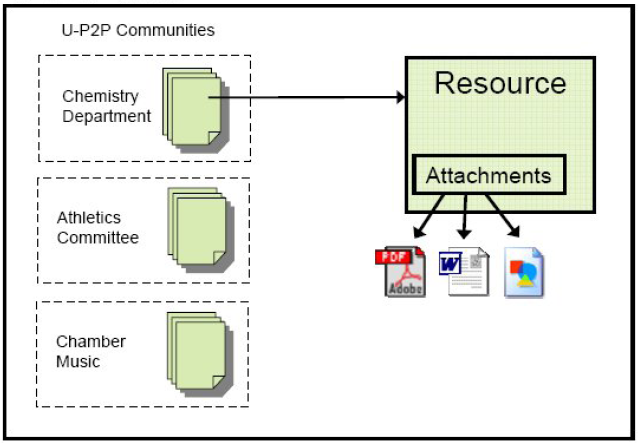
\includegraphics[width=0.75\textwidth]{img/comm_ex_diagram.png}
  \caption{A U-P2P user can be a member of many different communities.}
  \label{fig:CommDiagrram}
\end{figure}

% ------------------------------- UNIVERSAL PEER TO PEER NETWORKS -------------------------------

\section{Universal Peer to Peer Networks}

U-P2P uses the Gnutella protocol v 0.6. The Gnutella protocol is a peer-to-peer network protocol governed by the GNU license. U-P2P uses the JTella library created by Ken McCrary (versions up to 0.7), improved by Dan Meyer, (v 0.8), and finally modified and debugged by IBK Ajila. (v 0.9). The source of this JTella library is also available on the \href{http://sourceforge.net/projects/u-p2p/}{project SourceForge page}. 

A peer-to-peer community working with this protocol is fully decentralized (i.e there is no central server anywhere which indexes the resources shared on the network). Network issues such as how to discover existing communities or peers are not addressed in this user guide or in general in the publications about U-P2P.

% ------------------------------- GETTING STARTED -------------------------------

\section{Getting Started}

U-P2P is deployed as a web application within a JavaServer Pages (JSP) / Servlet engine (\href{http://tomcat.apache.org/}{Apache Tomcat}). The U-P2P client interface is accessed through a web browser. The web container listens to HTTP requests on a certain port (8080 under the standard U-P2P/Tomcat deployment), and routes those requests to the applications that are running within the container. The web server maps the URLs used for the requests to specific applications, and within these applications to specific servlets or JSP pages which handle the request and respond with HTML web pages.

To deploy U-P2P Apache Tomcat must first be installed. A default install of Apache Tomcat is included in the U-P2P deployed binaries. U-P2P must then be deployed to the Apache Tomcat "webapps" folder. To access the U-P2P interface navigate to the URL "/up2p/" on the Apache Tomcat server (ex. \href{http://inm-04.sce.carleton.ca:8080/up2p/}{http://inm-04.sce.carleton.ca:8080/up2p/} is the URL of the standard demo node).

\subsection{System Requirements}

In order to run and access U-P2P you can use:

\begin{itemize}
\item Windows 2000, Windows XP SP2 (or later), or Linux \footnotemark
\item \href{http://tomcat.apache.org/}{Apache Tomcat} version 5.5. U-P2P development and deployed binaries use Apache Tomcat 5.5.27.
\item The Java 2 Platform, Standard Edition (J2SE) \href{http://java.sun.com/javase/downloads/widget/jdk6.jsp}{Development Kit (JDK) 1.6.0} or higher.
\item A compatible web browser (\href{http://www.mozilla.com/en-US/firefox/}{Mozilla Firefox} is recomnmended). Cross browser compatibility is not a primarily goal of U-P2P and U-P2P is primarily tested with Firefox v4.
\end{itemize}
\footnotetext{U-P2P has successfully been tested on Windows 2000, Windows XP SP2, Windows 7, Linux Fedora and Kubuntu. No other operating systems have been tested by the development team. In theory, U-P2P should be compatible with any system which is supported by the Java 1.6 JDK and Apache Tomcat}


\newpage
\subsection{Universal Peer to Peer Distributions}

U-P2P is available in two regularly released distributions:

\begin{itemize}
\item 
\textbf{Binary Distribution (deployed in Apache Tomcat v5.5)}\\
The binary distribution consists of the following parts:\\
Web Container (Apache Tomcat v 5.5.27)\\
Universal Peer to Peer (deployed within tomcat)\\
Apache Xindice XML Database (deployed within tomcat)\\
\item
\textbf{Source Code Distribution}\\
The source code distribution is a stable release of the U-P2P and needs to be compiled and deployed to an Apache Tomcat web server, which is not included in the download package. Note that the Apache Xindice XML database is included with the source code and is automatically deployed by the build script along with U-P2P. For more details in the source code of U-P2P please see the Universal Peer to Peer Developer's Guide.
\end{itemize}

The U-P2P source code is also accessible directly from \href{http://sourceforge.net/projects/u-p2p/}{SourceForge} using an subversion (SVN) repository client. However, code saved during ongoing development may not function as described in this guide, if it functions at all. 

% ------------------------------- INSTALL FROM BINARY -------------------------------

\subsubsection{Installing U-P2P From the Binary Distribution}

\begin{enumerate}
\item 
Ensure the Java Development Kit is installed and the JAVA\_HOME environment variable points to the JDK directory e.g. set JAVA\_HOME=C:\textbackslash Program Files\textbackslash Java\textbackslash jdk1.6.0\_10). Note: a Java Runtime Environment (JRE) is not sufficient.
Please see section \ref{sec:JdkTrouble} for more details about JDK / JRE and setting environment variables.

\item
Download the U-P2P binary distribution from the project's \href{http://sourceforge.net/projects/u-p2p/files/}{SourceForge downloads page}. Unzip the package to a directory of your choice.

\item
\textbf{Important:} U-P2P is configured by default to attempt a connection to the standard demo node. This can be adjusted by modifying\\ "$<$Install Directory$>$\textbackslash Tomcat\textbackslash webapps\textbackslash up2p\textbackslash data\textbackslash HostCache.xml". For further information on how to configure U-P2P see section \ref{sec:Up2pConfig}.
\end{enumerate}

% ------------------------------- INSTALL FROM SOURCE -------------------------------

\subsubsection{Installing U-P2P From the Source Distribution}

\begin{enumerate}
\item
Ensure the Java Development Kit is installed and the JAVA\_HOME environment variable points to the JDK directory e.g. set JAVA\_HOME=C:\textbackslash Program Files\textbackslash Java\textbackslash jdk1.6.0\_10). Note: a Java Runtime Environment (JRE) is not sufficient.
Please see section \ref{sec:JdkTrouble} for more details about JDK / JRE and setting environment variables.

\item
Download the U-P2P source distribution from the project's \href{http://sourceforge.net/projects/u-p2p/files/}{SourceForge downloads page}. Unzip the package to a directory of your choice. The source code will be found in the "up2p\textbackslash src" directory, the relevant libraries in "up2p\textbackslash lib", and an empty "up2p\textbackslash build" directory is meant to receive the compiled code before it is deployed. The "up2p\textbackslash web" directory contains the JSP and configuration files for the up2p web application, as well as the Apache Xindice XML Database deployment.

\item
To build U-P2P, we have provided an Apache Ant build script ("up2p\textbackslash build.xml"). You can run this build file through Eclipse or using the \href{http://ant.apache.org/}{Apache Ant tool} directly. When running the Ant script the value of the variable catalina.home should be the path of the Apache Tomcat installation, and this way U-P2P will be deployed directly to Apache Tomcat:
	\begin{itemize}
	\item
	Under Eclipse, right-click on build.xml, and select �Run As$>$Ant build...� and you will see the Ant menu appear. In the �properties� tab, add a property called �catalina.home� and set it to the directory 	where your Apache Tomcat is installed. Under windows, use slashes as if in Linux (e.g. /C:/Program Files/apache-tomcat-5.5.26/). Then save and click �run� to build and deploy U-P2P to Tomcat. 
	\item
	To use Apache Ant directly, place yourself in the "up2p" directory (where the build.xml script is) and type the following command (assumes the Ant executable is already on the system PATH):
	\begin{verbatim}ant -Dcatalina.home="<tomcat home directory>"\end{verbatim}
	\end{itemize}
	
\item
\textbf{Important:} U-P2P is configured by default to attempt a connection to the standard demo node. This can be adjusted by modifying\\ "$<$Install Directory$>$\textbackslash Tomcat\textbackslash webapps\textbackslash up2p\textbackslash data\textbackslash HostCache.xml". For further information on how to configure U-P2P see section \ref{sec:Up2pConfig}.

\end{enumerate}

\subsection{Running Universal Peer to Peer}
Navigate to "$<$Install Directory$>$\textbackslash Tomcat\textbackslash bin" and execute startup.bat (Windows), or sh startup.sh (Linux) to start Tomcat and U-P2P. Note: Under Linux you may need to change the permissions associated with the sh files to make them executable.

Open a web browser and point it to "http://localhost:8080/up2p/". UP2P will initialize then initiate a redirect to the View page in the Root Community. Click on Create and Search to perform these activities (also see section �Features�, for details on the usage of U-P2P).

\subsection{Connection To Additional Hosts}

In order to setup a U-P2P network each peer in the network must have a connection to at least one other peer. Peers will automatically route network requests to all other peers they are connected to, so a direct connection between all peers in the network is not required. To connect to an existing peer the IP address of the existing peer must be added to the host cache configuration file. Please see section \ref{sec:HostCache} for more details on how to do this. If U-P2P is installed on two machines and the sample community described in section \ref{sec:SampleComm} has been created it will be possible to share the community definition and the community resources between the two nodes. 

\subsection{Stopping Universal Peer to Peer}

The scripts to terminate the Apache Tomcat server are located in "$<$Install Directory$>$\textbackslash Tomcat\textbackslash bin". To shutdown the server execute shutdown.bat (Windows) or shutdown.sh (Linux).

\textbf{Known Issue:} In some cases (particularly under Linux) U-P2P prevents the complete termination of Apache Tomcat and makes it impossible to restart U-P2P afterwards. In order to fully stop U-P2P it may be necessary to locate and kill the Java process (exercise caution if other Java applications are running on your computer).

% ------------------------------- FEATURES -------------------------------

\section{Universal Peer to Peer Features}
\label{sec:Features}

U-P2P presents three basic activites that involve the XML resources shared on the network: "Create", "View" and "Search". The complex query generator is also available through the "Query" activity, but this feature is in active development and likely to be unstable. Each of these features is accessible in the web browser interface provided with U-P2P. Start U-P2P and navigate a web browser to "http://localhost:8080/up2p" to access the main U-P2P interface.

\begin{figure}[h]
  \centering
  	\setlength\fboxsep{1pt}
		\setlength\fboxrule{1pt}
		\fbox{
    	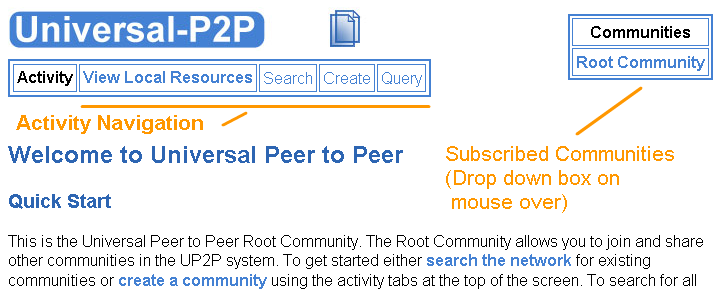
\includegraphics[width=\textwidth]{img/up2p_main.png}
    }
  \caption{The U-P2P standard header interface.}
  \label{fig:Up2pMain}
\end{figure}

Figure \ref{fig:Up2pMain} shows the standard interface header of U-P2P. Any activity can be selected and performed on the currently active community (shown in the community selection box when it is not focused). Click on the name of any community in community selection box to switch communities.

\subsection{Create}

Resources enter the U-P2P system through one of two ways:
\begin{itemize}
\item A user can complete an HTML form and submit it to U-P2P, where the data is compiled into an XML file.
\item The user can upload a ready-made XML file to the system.
\end{itemize}

In either case the XML file is processed, assigned a resource ID (based on a hash of the XML contents) and published/shared on the network in the active community.

\textbf{To create a resource:}

\begin{enumerate}
\item Select a community from the community selection box.
\item Click on the Create link to go to the create page for that community.
\item Fill out the create form or upload a file using the direct upload form at the top of the page (To access to direct upload form click on "Upload an Existing Resource". After clicking on the Upload/Create button you will be redirected to view the newly created resource.
\end{enumerate}

Uploaded files are stored within the directory \\
"$<$Install Directory$>$\textbackslash Tomcat\textbackslash webapps\textbackslash up2p\textbackslash community\textbackslash $<$Community ID$>$".

\subsection{View}
Resources in U-P2P are simply XML files that reside in the peer's database. To view them an XSLT stylesheet is used that transforms the plain XML (and any attachments) into a web page that can be viewed in a web browser. The stylesheet for viewing resources is specific to each community and like the Create page, it is provided by the community creator when the community is created. If no stylesheet is provided, a default stylesheet will attempt to render the resource in the web browser. 

\subsection{Search}
Searches in U-P2P are restricted to one community and are composed of query terms assembled on the Search web page. The Search page is provided by the creators of a community and is a basic HTML form that is submitted to U-P2P. For example, a user in a book community might have fields on their Search page for title, author and publisher. These would be filled out by the user and submitted to U-P2P. U-P2P will use the Network Adapter to perform the search and return the results to the user.

If you want to search for all the resources available in the community, simply type the wildcard star character (*) in a field of the search form.

\subsection{Query}
The query activity is used to access to complex query generator. This is used to perform relational queries on communities that support U-P2P URI links. This feature is in active development and is unsupported in this release. The generator is used to specify a set of relationships that a target resource must successfully match to appear in the results of the search. At each stage of the relationship chain the XPath to the linking attribute in the resource XML must be supplied. Each stage of the query can either search for incoming links to a resource or outgoing links to a resource. At this time not all possible generated queries are supported and as such search results may not always accurately reflect the results of a query.

\subsection{Joining A Community}
To join a community search in the Root Community and click on the Download link of a search result. This causes U-P2P to download the community XML file along with all associated attachments. The new community should be listed in the community selection box and you can enter it by clicking on the community title. Remember that a community is just like any other resource except that it is only found in the Root Community.

\subsection{Creating a Community}
For information on creating a community please see the Universal Peer to Peer Community Creation Reference.

% ------------------------------- TESTING -------------------------------

\section{Testing Universal Peer to Peer With Provided Samples}
\label{sec:SampleComm}

Some sample communities and resources are provided for testing purposes. Some of these come pre-installed with the binary distribution, and the complete set can be found in the "Test Data" directory at the top level of the binary package. In the source distribution these sample resources are found in the "test" subdirectory.

For this example U-P2P the Code Exchange sample community will be used to share snippets of program code. The following steps will guide you through the process of configuring and using the Code Exchange sample community. For more detailed information on the features of U-P2P see section \ref{sec:Features}

\begin{enumerate}
\item
In the U-P2P Root Community select the "Create" option. A new form will appear where the community definition can be specified or the complete XML definition can be directly uploaded (not used in this example).
\item
Specify the following properties for the community (Note: All files can be found in the test data directories specified above):
	\begin{center}
	\begin{tabular}{| l | l |}
		\hline
		\textbf{Attribute} & \textbf{Value} \\ \hline \hline
		Filename & code\_exchange.xml \\ \hline
		Title & Code Exchange \\ \hline
		Short Name & CodeExchange \\ \hline
		Category & Programming \\ \hline
		\multirow{2}{*}{Description} & A community for sharing short snippets of program
		\\ & code in any language. \\ \hline
		Keywords & Programming Code Snippet \\ \hline
		Title Location & /CodeSnippet/Title \\ \hline
		Community Display XSL Stylesheet & \\ \hline
		Resource Display XSL Stylesheet & code-res-view.xsl \\ \hline
		Display CSS & code-style.css\\ \hline
		Search Page & \\ \hline
		Search CSS & \\ \hline
		Create Page & code\_create.html\\ \hline
		Create CSS & code-style.css\\ \hline
		XML Schema & CodeSnippet.xsd\\ \hline
		Support Files\footnotemark
 & prettify.js (Javascript to support pretty printing)\\ \hline
	\end{tabular}
	\end{center}

\footnotetext{Note that a "Support File" can be any arbitrary attachment, and these files are shared with any peer that subscribes to the community. Although the code snippets in this example do not have an attachment, resource attachments function in much the same way as community support files.}

In this case not all the community definition fields need to be supplied. The community schema is simple enough that the standard U-P2P dynamically generated search page should be sufficient for the community's needs.
\item
Click �Submit�. You should now see the new document that you have created in the Root Community, and a new community called �Code Exchange� in the Root Community local repository and in the community selection box in the top right.

\item
Select the community �Code Exchange� in the community selection box. If you click on �View Local resources� you will see that you don't share any resources in this community yet. We will now create one.

\item
Select the �Create� activity from the tabs at the top of the screen. You should now view the customized create page of the Code Exchange community.

\item
For this example a resource will be created that describes a very simple bubble sort algorithm written in Java. Fill out the create form with the following fields:

\begin{center}
	\begin{tabular}{| l | p{0.75\textwidth} |}
		\hline
			\textbf{Attribute} & \textbf{Value} \\ \hline \hline
			Filename & bubble\_sort.xml \\ \hline
			Title & Bubble Sort \\ \hline
			Language & Java \\ \hline
			Author & U-P2P Test User \\ \hline
			Snippet &
				\begin{verbatim}
				public static void bubbleSort1(int[] x) {
			  	int n = x.length;
			  	for (int pass=1; pass < n; pass++) {
			    	for (int i=0; i < n-pass; i++) {
			      	if (x[i] > x[i+1]) {
			      		// Exchange elements
			        	int temp = x[i];  x[i] = x[i+1];  x[i+1] = temp;
			     		}
			    	}
			 		}
				}
				\end{verbatim} \\ \hline
				
	\end{tabular}
	\end{center}
	
\item
Submit the form. The new resource will appear with the rendering specified by the community definition. In this case Javascript is used to provide automatic syntax highlighting to the code sample.
\end{enumerate}

% ------------------------------- CONFIGURATION -------------------------------

\section{Configuration of Universal Peer to Peer}
\label{sec:Up2pConfig}

\subsection{Host Cache}
\label{sec:HostCache}

\textbf{Important:} As of U-P2P v3.3, all host cache configuration can be performed through the network status page, which is available at "http://localhost:8080/up2p/network-status.jsp" (when accessing U-P2P from the locally). This page can also be accessed by clicking on the number of connected peers in the top right of the web interface at any point.

In order to modify the peers that U-P2P attempts to connect to on startup edit the file "HostCache.xml" in the directory "$<$Install Directory$>$\textbackslash Tomcat\textbackslash webapps\textbackslash up2p\textbackslash data".

The contents of the file look like this:

\begin{SaveVerbatim}{verb:HostCacheExample}
<?xml version="1.0" encoding="UTF-8"?>
<HostCache>
	<host ip="inm-04.sce.carleton.ca" port="6346" />
</HostCache>
\end{SaveVerbatim}
\fbox{
	\BUseVerbatim{verb:HostCacheExample}
}

Each line of "$<$host ip="x.x.x.x" port="xxxx" /$>$" specifies a peer to connect to. Replace the existing entry with the IP address of the peer you want to connect to, or add more entries to initiate connections to multiple peers. You can add more hosts by inserting new such lines before the closing $<$/HostCache$>$ tag.

\textbf{Known Issue:} U-P2P requies at least one valid host cache entry to start up properly. As long as a host is specified it does not matter if the address is actually available.

Note that the default listening port of any peer is 6346. This is \textbf{not} the port that accepts browser requests. This is the port for network connections in between peers.

\subsection{Web Application Properties}
\label{sec:WebXml}

The web application configuration file for U-P2P can be found at \\"$<$Install Directory$>$\textbackslash Tomcat\textbackslash webapps\textbackslash up2p\textbackslash WEB-INF\textbackslash web.xml". End users should configure the "Access Filter" portion of this file, which appears as follows:
-
\begin{SaveVerbatim}{verb:WebXmlExample}
<filter>
	<filter-name>AccessFilter</filter-name>
	<description>Restricts access to the U-P2P client.</description>
	<filter-class>up2p.servlet.AccessFilter</filter-class>
	<init-param>
		<param-name>allow_remote_access</param-name>
		<param-value>false</param-value>
	</init-param>
	<init-param>
		<param-name>force_IP</param-name>
		<param-value>134.117.60.83</param-value>
	</init-param>
	<init-param>
		<param-name>tomcat_port</param-name>
		<param-value>8080</param-value>
	</init-param>
</filter>
\end{SaveVerbatim}
\fbox{
	\BUseVerbatim{verb:WebXmlExample}
}

\begin{description}
\item[allow\_remote\_access] \hfill \\
Determines whether the web interface can be accessed by non-local users. This defaults to false for security reasons. Valid values are: true, false
\item[force\_IP] \hfill \\
Deprecated: Previously, this field was used to specify the public IP address of the hosting machine. This configuration is no longer required as of U-P2P v3.3.
\item[tomcat\_port] \hfill \\
This determines the port that U-P2P will use the serve attachment files from. This should match the configured Apache Tomcat port (see section \ref{sec:TomcatPort}).
\end{description}

\subsection{Apache Tomcat Local Port}
\label{sec:TomcatPort}

U-P2P currently uses the Apache Tomcat 5.5 Java Servlet engine included in the U-P2P download package. It is configured to listen for incoming connections on port 8080. If other installations of Tomcat or other services are already using port 8080 U-P2P and Tomcat can be configured to use a different port (see section \ref{sec:WebXml} for instructions on modifying the U-P2P web application configuration).

\begin{enumerate}
\item
Edit "$<$Install Directory$>$\textbackslash Tomcat\textbackslash conf\textbackslash server.xml" and change the port attribute in the first Connector section (non-SSL Coyote HTTP/1.1 Connector).
\item
To access U-P2P navigate to "http://localhost:X/up2p", where X is chosen port number.
\end{enumerate}

\subsection{Logging}
U-P2P uses the Log4J logging system. The log files are found in the directory \\"$<$Install Directory$>$\textbackslash Tomcat\textbackslash webapps\textbackslash up2p\textbackslash log\textbackslash".
In order to configure the logging level or any logging properties, the master configuration file is "log4j.properties", found in the source directory "src\textbackslash up2p\textbackslash core\textbackslash", and specific logging for the JTella adapter is found in the file 
\\"up2p.peer.jtella.log4j.properties" in the directory "src\textbackslash up2p\textbackslash peer\textbackslash jtella\textbackslash". Note that on deployment of the application  these files are copied to the corresponding class directory under \\"$<$Install Directory$>$\textbackslash Tomcat\textbackslash webapps\textbackslash up2p\textbackslash WEB-INF\textbackslash classes\textbackslash".
The logging level is set by default to �DEBUG�. If you want to see less logs, set it to �INFO� or �ERROR�. If you want to see only a minimal amount of logs, you can change the level to �FATAL�.

% ------------------------------- TROUBLESHOOTING -------------------------------

\section{Troubleshooting}
\subsection{Firewalls and Universal Peer to Peer}
U-P2P currently does not provide a means to transgress firewalls and allow sharing of resources between two fire walled peers. The local address and the Tomcat port (8080 by default) are used for all outgoing resource links and other peers will attempt to connect to this address when they retrieve your published resources. A firewall can be set up to forward these requests to a peer on an internal network. Consult your local administrator or the documentation included with your firewall / router to enable port forwarding of U-P2P requests. The required ports to forward are 8080 (for HTTP requests) and 6346 (for the Gnutella connection between peers).

\subsection{Java Environment}
\label{sec:JdkTrouble}

A Java Runtime Environment is not sufficient to run U-P2P (JSPs require active compilation). A \href{http://java.sun.com/javase/downloads/widget/jdk6.jsp}{Java Development Kit} (JDK) must be installed, and the JAVA\_HOME environment variable must point to the directory where the JDK is installed.

Note:

\begin{itemize}
\item Generally on installing the JDK the JAVA\_HOME environment variable is automatically set to the appropriate directory.
\item The binary release of U-P2P was compiled using Java 1.6 SE, so you will need this version of the JDK or higher. You may, however, compile the source distribution with Java 1.5, and then run it with this version (unsupported).
\end{itemize}

Setting environment variables in Windows 95/98/Me/NT/2000/XP:
\begin{itemize}
\item
In Windows 95/98/ME, append these lines to the end of  "C:\textbackslash autoexec.bat" using notepad, and reboot:
 
set JAVA\_HOME=C:\textbackslash Program Files\textbackslash Java\textbackslash jdk1.6.0\_10\\  (Replace with appropriate directory)
\end{itemize}
In Windows NT/2000/XP, follow the following steps:
\begin{enumerate}
\item Open Control Panel 
\item Click the System icon and the window pops up (If the System icon does not appear try switching to the Control Panel classic view).
\item Navigate to the Advanced pane
\item Click the Environment Variables button
\item There are two separated windows showing two sets of environment variables. The top window shows variables specific to the user, the bottom one show global environment variables. Select the "New" button to create a new environment variable. Select the "Edit" button to edit an existing environment variable.
\end{enumerate}

% ------------------------------- SCHEMA TOOL -------------------------------

\section{SchemaTool}

SchemaTool is a separate project that was developed to allow easy authoring of XML Schema without having any knowledge of the language. It allows anyone to create a simple schema using a wizard-type interface and provides support for built-in and derived data types.
You can create a schema in SchemaTool and save the file using the Download feature to a local file that you can attach to your U-P2P community.

\begin{figure}[h]
  \centering
  	\setlength\fboxsep{1pt}
		\setlength\fboxrule{1pt}
		\fbox{
    	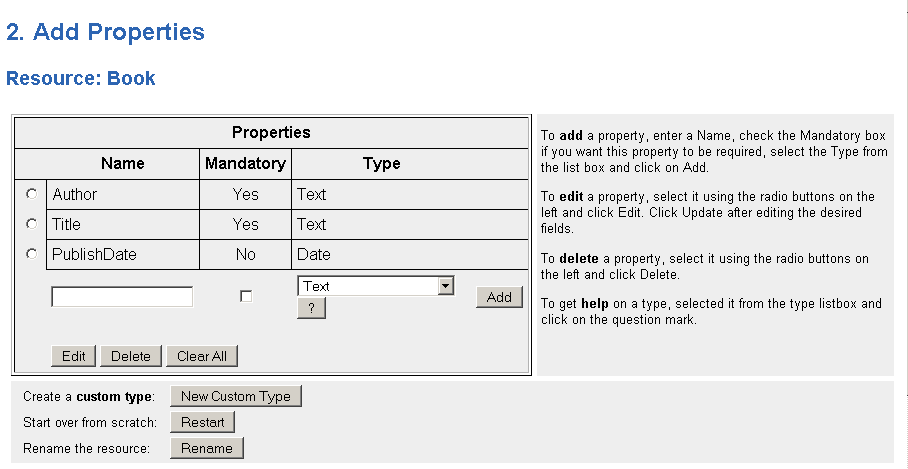
\includegraphics[width=\textwidth]{img/schematool.png}
    }
  \caption{The SchemaTool XML Schema Wizard.}
  \label{fig:SchemaTool}
\end{figure}

SchemaTool is limited to simple XML structures but provides excellent support for describing resources using a flat list of properties. For example, a book resource might have an author, title, and date of publication. These properties can be quickly added to a schema and the publication date set to use the 'Date' data type. The schema would then be downloaded to a local file. When creating a new community, the community schema would be set to the schema that was just created in SchemaTool (by manually browsing to find the downloaded file).

% ------------------------------- MORE INFORMATION -------------------------------

\section{More Information}
Universal Peer-to-Peer is an open source project hosted on SourceForge and developed in the Department of Systems and Computer Engineering at Carleton University in Ottawa, Canada. Further documentation can be found in the Universal Peer to Peer Developer�s Guide and the Universal Peer to Peer Community Creation Reference available at the U-P2P Home Page.

A number of helpful resources are available online:

\begin{center}
	\begin{tabular}{| p{0.4\textwidth} | p{0.6\textwidth} |}
		\hline
			\textbf{Documentation} & \textbf{Notes} \\ \hline \hline	\href{http://sites.google.com/a/nmai.ca/home/research-projects/universal-peer-to-peer-home}{U-P2P Home Page} & The central source for all things U-P2P. It contains the latest news, links and downloads for the entire project. \\ \hline
			\href{http://sourceforge.net/projects/u-p2p/}{U-P2P Project Page} & The SourceForge Project Page provides a summary of the status of development and the latest code releases. \\ \hline
			\href{http://sourceforge.net/forum/?group_id=17676}{U-P2P Forums} & Post your question in a forum since it might be a common problem. Suggestions and feature requests are welcome. \\ \hline
			\href{http://tomcat.apache.org/tomcat-5.5-doc/index.html}{Tomcat 5.5 Documentation} & Docs for Tomcat can help resolve any problems in starting Tomcat or using UP2P in conjunction with an existing Tomcat installation. \\ \hline
			\href{http://www.w3.org/XML/}{Extensible Markup Language (XML)} & The home page for the XML standard and related documentation. \\ \hline
			\href{http://www.w3.org/Style/XSL}{Extensible Stylesheet Language Transformations (XSLT) 1.0} & The Style home page has links to the full specification of XSLT and other related tools and material. Note that XSLT 2.0 is currently \textbf{not} supported by U-P2P \\ \hline
			\href{http://www.w3.org/XML/Schema}{XML Schema} & The Schema home page has the specifications and links to useful free XML Schema validation services. \\ \hline
	\end{tabular}
\end{center}

There is room for improvement in both the implementation of U-P2P and the U-P2P theoretical framework in general. All suggestions will be carefully considered and can be posted to the U-P2P Feature Request or Forums on SourceForge.net or e-mailed directly to the contacts listed on the U-P2P Home Page.

\end{document}